\chapter{Preliminaries}
\epigraph{
  I can't go to a~restaurant and order food because I keep looking at the fonts on~the menu.
}{Donald Knuth}
Let us start with some games\ldots

\section{Game Theory}
\epigraph{
  You have to learn the rules of~the game.
  And then you have to play better than anyone else.
}{Albert Einstein}
Game theory is a~mathematical discipline dealing with interactions (either conflicts or cooperation) between $2$ or more agents.
Founded by (\cite{VonNeumann1953theory}), game theory has countless application in~economics, political science, and psychology, as well as~logic, computer science, biology and Poker.

Informally, a~\emph{game} has typically
\begin{itemize}
  \item players, who are assumed to be rational decision-makers, i.e. they would not make a~suboptimal choice of~actions,
  \item actions available to each player,
  \item payoffs (or utilities) for every possible combination of~such actions.
\end{itemize}

Games can be represented in~two forms:
\begin{itemize}
  \item \acrfull{nfg} is a~representation using (pay-off) \emph{matrices}.
    Examples of~\acrshort{nfg}s can be found in Section~\ref{sec:examples-of-games}.
  \item \acrfull{efg} represents a~\emph{game with turns} using a~\emph{game tree}.
    They are discussed in greater details in~Section~\ref{sec:extensive-form-perf-info} and Section~\ref{sec:extensive-form-imperf-info}.
\end{itemize}

\section{Examples of~Games}
\label{sec:examples-of-games}
\epigraphLong{
  Happy Hunger Games!
  And may the odds be ever in~your favor.
}{Suzanne Collins, \emph{The Hunger Games}}
\newcommand{\figurewidthratio}{0.3}
\begin{description}
  \item [\acrfull{rps}] is a~game commonly used to make decision between two people.
    Two players pick a~(symbolical) tool of~their choice: Rock, Paper or Scissors.
    Each tool wins against one of~the remaining tools and loses against the other one: Scissors cuts Paper, Paper covers Rock and Rock crushes Scissors (check also Section~\ref{sec:intricate-ex}).

  \item [Chess] is arguably world's most famous game, frequently employed to sharpen one's intellectual facilities.
    For decades, this mind sport has functioned as a~``playground'' for \acrfull{ai} research.

    The most notable milestone of~computer Chess took place in New York City in 1997:
    the~\acrshort{ai} community (as well as the rest of~the world) was astonished by the victory of~IBM's computer system \emph{Deep Blue} against the world champion, the grandmaster \emph{Garry Kasparov}.
    \epigraphLong{
      It was an~impressive achievement, of~course, and a~human achievement by~the members of~the IBM team, but Deep Blue was only intelligent the way your programmable alarm clock is intelligent.
      Not that losing to a~\$10 million alarm clock made me feel any better.
    }{Garry Kasparov}
    The rules of~Chess are widely known; for completeness, however, I recommend tutorial (\cite{Karpov1997disney}) for introduction to Chess.

  \item [Go] is another ancient game with countless number of~both amateur and professional players.
    The rules (Section~\ref{sec:Go}) are even simpler than in Chess; yet the game is far more complex, with the number of~positions greater than the count of~atoms in the Universe (Section~\ref{sec:game-tree-search}).

    As a~game of intellect, Go is especially popular with mathematicians.
    A~dedicated mathematical discipline of~\acrfull{cgt} was developed by respected John Conway, in order to decompose and study endgame positions (Chapter~\ref{ch:goCGT}).

    Finally, the Go world experienced a~duel similar to the one of~Deep Blue vs. Kasparov.
    The Humanity, represented by legendary Korean player Lee Sedol, was defeated by the~\acrshort{ai} of~Google DeepMind's program \emph{AlphaGo} (Chapter~\ref{ch:AlphaGo}).

  \item [Nim] is a~mathematical game in which two players take turns in~removing objects from distinct heaps.
    On each turn, a~player must remove at~least one object, and may remove any number of~objects provided they all come from the same heap.
    The goal is to be the player to remove the last object.

  \item [Poker] is a~popular card game\footnotemark{} and an~example of~an~imperfect-information game: as opposed to~all previous games, players' \emph{private} cards and the \emph{chance} play vital roles here.
    \footnotetext{For the rules of~Poker, read Section~\ref{sec:Poker}.}
    We will see that notion of~a~subgame needs to be adapted for imperfect-information games, which will cause several complications and will call for novel solutions (Part II).

    Following the examples of~Deep Blue and AlphaGo, the world had a~chance to meet a~superhuman \acrshort{ai} champion as well in Poker.
    \emph{Cepheus} is the first Poker-bot that has \emph{weakly solved} \acrlong{lhe} variant of~Poker (\cite{Bowling2015heads}).
\end{description}

\note{
  The following examples and figures are taken from the classic textbook \emph{Algorithmic Game Theory} (\cite{AGT07}).
}

\epigraphLong{
  Football is a~more beautiful game in~high definition.
}{José Mourinho}

\begin{description}
  \item [Matching Pennies] is a~$2$-choice version of~\acrshort{rps}.
    Two players, \emph{Matcher} and \emph{Mismatcher}, toss two coins (pennies).
    If the coins match, Matcher wins (receives the utility of~$1$) and Mismatcher loses (receives the utility of~$-1$).
    If the coins mismatch, Mismatcher wins and Matcher loses.
    \begin{figure}[H]
      \centering
      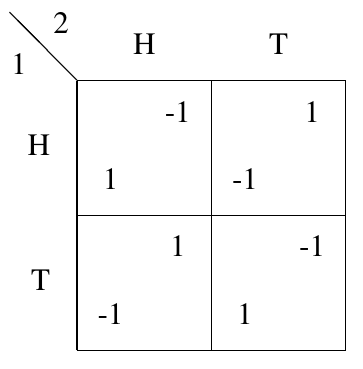
\includegraphics[width=.3\textwidth]{../img/matching-pennies.png}
      \caption[Matching Pennies]{Matching Pennies: player~$1$ as the Matcher, player~$2$ as the Mismatcher \\(\cite{AGT07})}
      \label{fig:matching-pennies}
    \end{figure}

  \item [Prisoner's Dilemma] is a~notorious example from game theory.
    Two players, prisoners, are on~trial for a~crime, each with choice to confess or to remain silent.

    If they both keep silence, charges against them cannot be proved, and both will serve a~short prison term of~2~years (for minor offenses).
    If just one of~them confesses, his term will be reduced to 1~year and he will be used as a~witness against the other, who in~turn will get a~sentence of~5~years.
    Finally, if they both confess, they both will get a~small relief for cooperation, and each will be sentenced to 4~years instead of~5.~(\cite[Section~1.1.1]{AGT07})
    \begin{figure}[H]
      \centering
      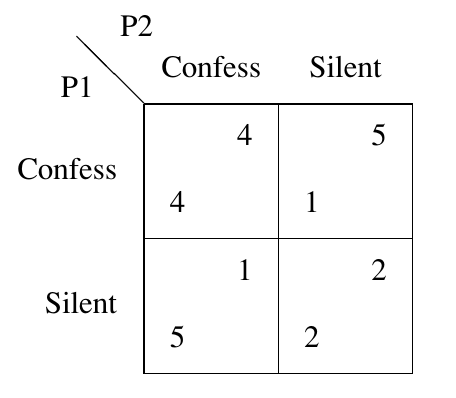
\includegraphics[width=.25\paperwidth]{../img/prisoner.png}
      \caption[Prisoner's Dilemma]{Prisoner's Dilemma (\cite{AGT07})}
      \label{fig:prisoner}
    \end{figure}
    The situation modeled by the Prisoner's Dilemma arises naturally in a~lot of~different situations.
    One such example is \acrshort{isp} Routing Game.

  \item [\acrshort{isp} Routing Game] models an~\acrfull{isp}, who needs to send Internet packets from source~$s_1$ (in his own network \acrshort{isp}1) to target~$t_1$ (in the network \acrshort{isp}2 of~another provider).
    The two networks are connected via two transit points, $C$ (for confess) and $S$ (for silent):
    \begin{figure}[H]
      \centering
      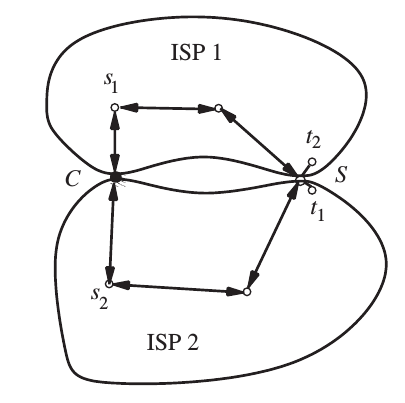
\includegraphics[width=.25\paperwidth]{../img/isp.png}
      \caption[\acrshort{isp} Routing Game]{\acrshort{isp} Routing Game (\cite{AGT07})}
      \label{fig:isp-routing}
    \end{figure}
    There is a~unit cost per edge:
    if the provider sends a~packet through $C$, it costs him $1$ unit and the opponent pays $4$ units for routing from $C$ to~$t_1$.
    \textbf{\acrshort{isp}1 possesses a~selfish behavior.}
    Otherwise, if he sends a~packet through $S$, it costs $2$ units.
    The opponent however pays only $1$ unit, because $t_1$ is closer to $S$ than to $C$.
    \textbf{\acrshort{isp}1 possesses an~altruistic behavior.}

    Now \acrshort{isp}2 will send traffic, too, choosing again between $C$ or $S$.
    If we accumulate all costs from both traffics, and write it down for each combination of~selfish/altruistic players, we get the identical \acrshort{nfg} as in Figure~\ref{fig:prisoner}.

  \item [Traffic Light]
    Two players, drivers of~cars, arrive at~a~crossroad perpendicularly to one another.
    If at most 1~driver crosses, the situation will be safe and their payoffs will be non-negative, with a~slightly better payoff for the passing player.
    If however both drivers decide to pass the crossroad, the result will be extremely sub-optimal, as both drivers obtain drastically negative payoffs and~die.

    \begin{figure}[H]
      \centering
      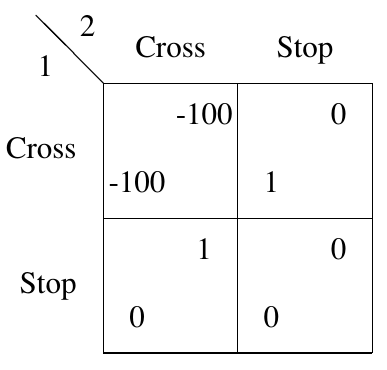
\includegraphics[width=.23\paperwidth]{../img/traffic-light.png}
      \caption[Traffic Light]{Traffic Light (\cite{AGT07})}
      \label{fig:traffic-light}
    \end{figure}

    This is an~example of~a~\emph{coordination game}, where a~common trusted \emph{coordination device} is desirable.
    Such a~device (e.g., a~traffic light or the right-of-way priority rule) justify the concept of~a~\emph{correlated equilibrium} (\cite[Subsection~1.3.6]{AGT07}).

  \item [Battle of Sexes] is another coordination game:
    Two players, Boy and Girl, are arranging an~activity for their date.
    The Girl wishes to go (S)hopping, while the Boy wants to go for a~(B)eer:
    \begin{figure}[H]
      \centering
      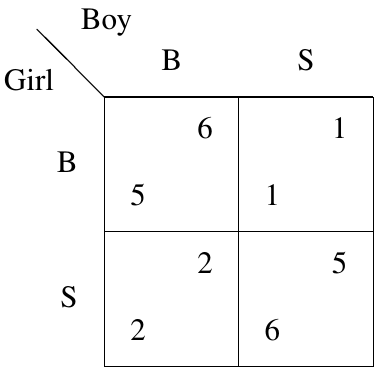
\includegraphics[width=.23\paperwidth]{../img/battle-of-sexes.png}
      \caption[Battle of~Sexes]{Battle of~Sexes (\cite{AGT07})}
      \label{fig:battle-of-sexes}
    \end{figure}
    Notice they both prefer to agree (rather than disagree) on~the activity, because this way they will be together.
    If however, they disagree and end up alone without a~date, both would rather spend the evening doing their favorite activity.
\end{description}

\section{The Game of Go}
\label{sec:Go}
\epigraphLong{
  You don't have to be really good anymore to get good results.
  What's happening with Chess is that it's gradually losing its place as the par excellence of~intellectual activity.
  Smart people in~search of~a~challenging board game might try a~game called~Go.
}{Hans Berliner}

\emph{Black} and \emph{White} place pieces (\emph{stones}) on the unoccupied intersections (\emph{points}) of a~\emph{board} with a~$19\times19$ grid of~lines.
Players take turns, Black moves first.
There are only 2 basic rules of Go:
\begin{description}
  \item [The rule of liberty]
    Every stone remaining on the board must have at least one open point (an~intersection, called a~\emph{liberty}) directly next to it (up, down, left, or right), or must be part of a~connected group that has at least one such liberty next to it.
    \begin{figure}[H]
      \centering
      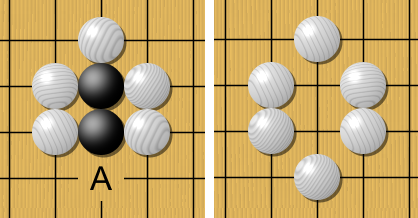
\includegraphics[width=.5\textwidth]{../img/Go_rule_of_liberty.png}
      \caption{The rule of liberty}
      \label{fig:Go-rule-liberty}
    \end{figure}

    Stones or groups of stones which lose their last liberty are removed from the board.

  \item [The ``ko'' rule]
    The stones on the board must never repeat a~previous position of~stones.
    This is to prevent unending cycles.
    \begin{figure}[H]
      \centering
      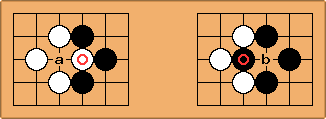
\includegraphics[width=.5\textwidth]{../img/Go_ko_rule.png}
      \caption{The ``ko'' rule}
      \label{fig:Go-Ko-rule}
    \end{figure}
\end{description}

There are several \textbf{scoring rules} to determine the winner of a~game.
In the match of~AlphaGo against Lee Sedol,%
\footnote{See Chapter~\ref{ch:AlphaGo}.}
the \emph{area scoring} was used.
Under area scoring system, player's score is:
\begin{itemize}
  \item the number of stones that the player has on the board
  \item plus the number of~empty intersections surrounded by that player's stones
  \item plus \emph{komi(dashi)} points%
    \footnote{a~compensation for the first move advantage of~the Black player}
    for the White player
\end{itemize}

\emph{Elo rating} can be used to denote players' \textbf{ranks}.
Alternatively, \emph{kyu/dan} (in~Japanese) or \emph{gup/dan} (in~Korean) system is also vastly popular:
\begin{table}[!htbp]
  \centering
  \begin{tabular}{ |l|r|l| }
    \hline
    \textbf{Rank Type} & \textbf{Range} & \textbf{Stage} \\
    \hline
    double-digit kyu\footnotemark{} (DDK) & 30--21k & beginner \\
    double-digit kyu                      & 20--11k & casual player \\
    single-digit kyu (SDK)                & 10--1k  & intermediate amateur \\
    amateur dan                           & 1--7d   & advanced amateur \\
    ~ & (8d is special title) & ~ \\
    professional dan                      & 1--9p   & professional player \\
    ~ & (10d is special title) & ~ \\
    \hline
  \end{tabular}
  \caption{Ranks in Go}
  \label{tab:Go-ranks}
\end{table}
\footnotetext{gup in Korean}

\textbf{Handicap} system is used to even up differences in ranks:
Black can place 1 or more stones in advance as a~compensation for White's greater strength.

\section{Combinatorial Game Theory}
\label{sec:CGT}
\todo

\section{The Game of~Poker}
\label{sec:Poker}
\epigraphLong{
  Each player must accept the cards life deals him or her:
  but once they are in~hand, he or she alone must decide how to play the cards in~order to win the game.
}{Voltaire}
Poker is a~card game played with a~\emph{pack} of~52 standard cards\footnotemark{} and tokens of~payment called \emph{chips}.
\footnotetext{$A\spadesuit$, $K\heartsuit$, $Q\clubsuit$, $J\diamondsuit$, \ldots}

There are many variants of~Poker, the two perhaps most popular ones are \acrfull{lhe} and \acrfull{nlhe}.
Two-player version of~\acrshort{nlhe} (Heads-Up \acrshort{nlhe}) is currently the game of~most active research in the computer Poker community (\cite{Ganzfried2015endgame}).

\begin{description}
  \item [Players:] \todo
    \begin{itemize}
      \item Small Blind
      \item Big Blind
    \end{itemize}

  \item [Actions:] \todo

  \item [Payoffs:] \todo 
\end{description}
\todo
